\noindent{\Huge\scshape И}{\LARGE\scshape стория}\\
\rule[0.5\baselineskip]{\textwidth}{1pt}

\vspace{0\baselineskip}

\subsection*{Задание 22.}
Прочти часть главы о Катоне Старшем из \textsl{«Сравнительных Жизнеописаний»} Плутарха. 
\vspace*{-18pt}{\sl\begin{quote} \end{quote}
Найдя Карфаген не в плачевном положении и не в бедственных обстоятельствах, как полагали римляне, но изобилующим юношами и крепкими мужами, сказочно богатым, переполненным всевозможным оружием и военным снаряжением и потому твердо полагающимся на свою силу, Катон решил, что теперь не время заниматься делами нумидийцев и Масиниссы и улаживать их, но что если римляне не захватят город, исстари им враждебный, а теперь озлобленный и невероятно усилившийся, они снова окажутся перед лицом такой же точно опасности, как прежде.
}\bigskip

Для полного ответа используй всю главу, посвященную Катону (http://ancientrome.ru/antlitr/t.htm?a=1439001800\#26)

Ответь на следующие вопросы:
\begin{list}{\asbuk{nnn})}{\usecounter{nnn}\leftmargin=6mm \labelwidth=5mm \topsep=0mm \labelsep=2mm \itemsep=0pt \parsep=0mm \itemindent=-1pt}
\item Какие события в личной истории Катона и всей Римской республики повлияли на решение о начале войне с Карфагеном? Ответ обоснуй примерами из указанного источника.
\item Плутарх указывает на ряд черт личности, которые способствовали успеху Катона Старшего. Выдели их из текста, укажи в ответе. С какой, по-твоему, целью автор пишет биографию Катона, как и прочих героев в своих «Сравнительных жизнеописаниях», в попарном сравнении?
\end{list}

\subsection*{Задание 23.}
Перед тобой картина Яна Матейко «Грюнвальдская битва» (1878) (см. рис.~\ref{matejko}, стр.~\pageref{matejko}). Рассмотри её детально и ответь на следующие вопросы.
    
\begin{list}{\asbuk{nnn})}{\usecounter{nnn}\leftmargin=6mm \labelwidth=5mm \topsep=0mm \labelsep=2mm \itemsep=0pt \parsep=0mm \itemindent=-1pt}
\item С чем связан выбор персонажей, изображенных на картине указанного сражения?
\item Обратись к дате создания работы. Укажи, почему автор обратился именно к данному сюжету. Сравни данную картину с другими полотнами того же художника: «Прусская дань», «Стефан Баторий под Псковом», «Конституции 3 мая».
\item Перечисли явления в общественной жизни, протекавшей на территории современной Польши во времена Российской империи, ставшие своего рода катализатором общественных настроений и событий, которые пан Матейка пытался передать в своих полотнах.
\end{list}   

\begin{figure}
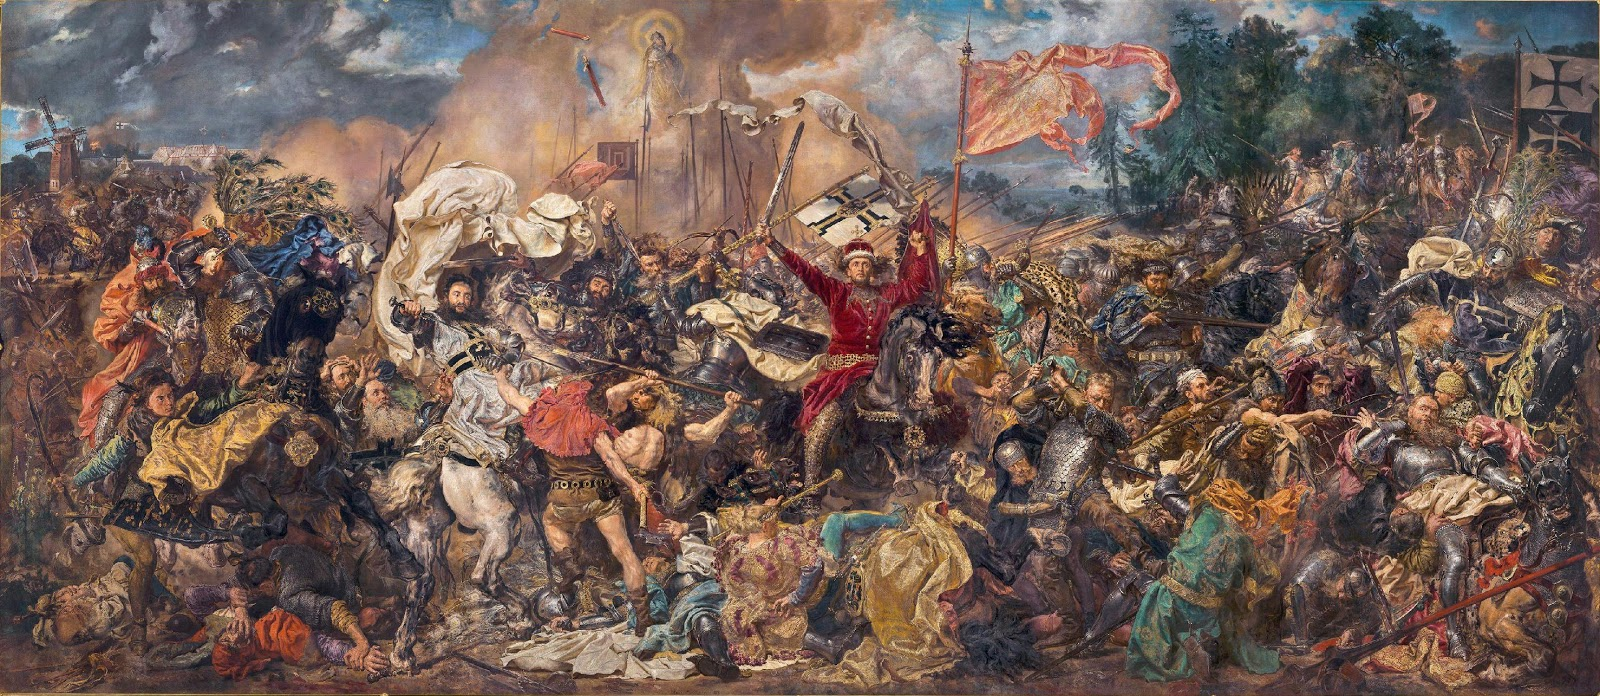
\includegraphics[width=1\textwidth]{images/history-2.jpg}\caption{\label{matejko}Грюнвальдская битва}
\end{figure}

\subsection*{Задание 24.}
    Перед тобой фрагмент иностранного документа о России «Muscovitica Extranea 156. 1». Сегодня данный документ хранится в Шведском государственном архиве. Прочитай его и ответь на следующие вопросы:
    
    \begin{enumerate}
    \item Укажи, о каком времени говорит источник. Аргументируй свою позицию цитатами из текста.
    \item В тексте курсивом выделен фрагмент (1). Укажи, с чем связано такое холодное отношение отца к сыну. Какие у них имена? Аргументируй свою позицию ссылками на источник. Используй позиции, предложенные историками (не более 1-ой).
    \item В тексте курсивом выделен фрагмент (2). Объясни необходимость данного действия в реалиях того времени. Опиши атмосферу, которую передает источник. Сильна ли власть царя? Где проявляются ее сильные стороны, а где – слабые? Что на это влияет? 
    \item Порассуждай, кто мог быть автором источника. Учитывай, что он/они обладает/ют сведениями о государственном устройстве, так же – перечнем имен, занятых в политике (спойлер: точного имени нет, но оно и не нужно).
    \end{enumerate}   
    
    «В Москве никакое важное дело не обсуждается без представления патриарху, отцу великого князя, не потому, что сие допускает религия, но потому, говорят, что отец заранее выговаривает это у сына. Его духовное имя <…>, мирское имя — <…>.
    \\
    Его бывшая супруга <…>, или <…>, тоже духовное лицо, или инокиня, но должна заботиться о домашних делах великого князя, своего сына, естественная любовь которого обращена более к матери, нежели к отцу, \textit{настолько, что отец и сын долгое время в Москве не встречались ($1$)}, и виной тому настоятельный совет отца, чтобы сын вступил в брак, но не со здешней девицей, а из Бранденбургского княжеского дома. Тогда мать изо всех сил воспротивилась этому и поклялась не давать никакого благословения сыну и все время, днем и ночью, хлопотала, чтобы поспеть первой, что и случилось; из сотен девиц во всей стране не нашла она более подходящей к этому званию, чем дочь князя <…>, и <…> c ней наскоро отпраздновали свадьбу. \textit{Свадьба праздновалась при запертых воротах города ($2$)}. Первые два дня прошли в обрядах, на третий день слышны были барабаны и сотни труб, на четвертый день были в печали все, кто находился в Москве: в тот же день терем, где он как раз находился, весь обрушился на задний двор и сгорел дотла.
    \\
    Наиболее знатные бояре, которые правят в Москве, суть следующие <…> [идет перечень имен и титулов]»

